\documentclass[12pt,spanish, american,b4paper, onecolumn, lmargin=1cm, rmargin=1cm, tmargin=1cm, bmargin=2cm,]{article}
\usepackage[T1]{fontenc}
\usepackage{lmodern}
\usepackage{amssymb,amsmath}
\usepackage{ifxetex,ifluatex}
\usepackage{fixltx2e} % provides \textsubscript
% use upquote if available, for straight quotes in verbatim environments
\usepackage{booktabs}				% suport to table rule EDB
\IfFileExists{upquote.sty}{\usepackage{upquote}}{}
\ifnum 0\ifxetex 1\fi\ifluatex 1\fi=0 % if pdftex
  \usepackage[utf8]{inputenc}
  \usepackage{eurosym}
\else % if luatex or xelatex
  \ifxetex
    \usepackage{mathspec}
    \usepackage{xltxtra,xunicode}
  \else
    \usepackage{fontspec}
  \fi
  \defaultfontfeatures{Mapping=tex-text,Scale=MatchLowercase}
  \newcommand{\euro}{€}
\fi
% use microtype if available
\IfFileExists{microtype.sty}{\usepackage{microtype}}{}
\usepackage[margin=1.45in]{geometry}
\usepackage{color}
\usepackage{fancyvrb}
\newcommand{\VerbBar}{|}
\newcommand{\VERB}{\Verb[commandchars=\\\{\}]}
\DefineVerbatimEnvironment{Highlighting}{Verbatim}{commandchars=\\\{\}}
% Add ',fontsize=\small' for more characters per line
\newenvironment{Shaded}{}{}
\newcommand{\KeywordTok}[1]{\textbf{{#1}}}
\newcommand{\DataTypeTok}[1]{\textcolor[rgb]{0.50,0.00,0.00}{{#1}}}
\newcommand{\DecValTok}[1]{\textcolor[rgb]{0.00,0.00,1.00}{{#1}}}
\newcommand{\BaseNTok}[1]{\textcolor[rgb]{0.00,0.00,1.00}{{#1}}}
\newcommand{\FloatTok}[1]{\textcolor[rgb]{0.50,0.00,0.50}{{#1}}}
\newcommand{\CharTok}[1]{\textcolor[rgb]{1.00,0.00,1.00}{{#1}}}
\newcommand{\StringTok}[1]{\textcolor[rgb]{0.87,0.00,0.00}{{#1}}}
\newcommand{\CommentTok}[1]{\textcolor[rgb]{0.50,0.50,0.50}{\textit{{#1}}}}
\newcommand{\OtherTok}[1]{{#1}}
\newcommand{\AlertTok}[1]{\textcolor[rgb]{0.00,1.00,0.00}{\textbf{{#1}}}}
\newcommand{\FunctionTok}[1]{\textcolor[rgb]{0.00,0.00,0.50}{{#1}}}
\newcommand{\RegionMarkerTok}[1]{{#1}}
\newcommand{\ErrorTok}[1]{\textcolor[rgb]{1.00,0.00,0.00}{\textbf{{#1}}}}
\newcommand{\NormalTok}[1]{{#1}}
\usepackage{graphicx}
% Redefine \includegraphics so that, unless explicit options are
% given, the image width will not exceed the width of the page.
% Images get their normal width if they fit onto the page, but
% are scaled down if they would overflow the margins.
\makeatletter
\def\ScaleIfNeeded{%
  \ifdim\Gin@nat@width>\linewidth
    \linewidth
  \else
    \Gin@nat@width
  \fi
}
\makeatother
\let\Oldincludegraphics\includegraphics
{%
 \catcode`\@=11\relax%
 \gdef\includegraphics{\@ifnextchar[{\Oldincludegraphics}{\Oldincludegraphics[width=\ScaleIfNeeded]}}%
}%
\ifxetex
  \usepackage[setpagesize=false, % page size defined by xetex
              unicode=false, % unicode breaks when used with xetex
              xetex]{hyperref}
\else
  \usepackage[unicode=true]{hyperref}
\fi
\hypersetup{breaklinks=true,
            bookmarks=true,
            pdfauthor={Eduardo B. Díez},
            pdftitle={Severe Weather Events in the United States:  Decisive Reasons},
            colorlinks=true,
            citecolor=magenta,
            urlcolor=blue,
            linkcolor=red,
            pdfborder={0 0 0}}
\urlstyle{same}  % don't use monospace font for urls
\setlength{\parindent}{0pt}
\setlength{\parskip}{6pt plus 2pt minus 1pt}
\setlength{\emergencystretch}{3em}  % prevent overfull lines
\setcounter{secnumdepth}{5}
\ifxetex
  \usepackage{polyglossia}
  \setmainlanguage{}
\else
  \usepackage[spanish, american]{babel}
\fi

\title{Severe Weather Events in the United States: \newline{} Decisive Reasons}
\author{Eduardo B. Díez}
\date{July 23, 2014}

\begin{document}

\begin{center}
\huge Severe Weather Events in the United States: \newline{} Decisive Reasons \\[0.2cm]
\large \emph{Eduardo B. Díez}\\[0.1cm]
\large \emph{July 23, 2014} \\
\normalsize
\end{center}

\renewcommand{\abstractname}{Synopsis}
\begin{abstract}
Using the Severe Weather Data (N=902297) from the National Oceanic and
Atmospheric Administration, we examined which types of events are most
harmful to population health and which have the greatest economic
outcomes during the years 1950 to 2011.

Significant differences were observed between the events with greatest
consequences to the population healt and to the economy.

Visually inspecting the tabulated data and graphs leads us to affirm
that floods are the major causes of damage to property and crops, and
tornadoes are responsible for large numbers of fatalities and injuries.
\end{abstract}

\section{Introduction}\label{introduction}

This report relates to explore the NOAA {[}3{]} Storm Database looking
for those weather events that are detrimental to population's health as
well as those who have the greatest economic consequences.

\begin{quote}
\begin{quote}
Few variables from the dataset were used and transformed to obtain a
wide table, with which to display a couple of plots giving response to
the issues this report deals. So, the output of the R-code developed and
included in \hyperref[datapro]{§ Data Processing}, is conformed by one
table and two plots that the interested reader could find at
\hyperref[results]{§ Results}
\end{quote}
\end{quote}

To complete the Peer Assessment 2 as requested for the course
\textbf{Reproducible Research} by Roger D. Peng, Jeff Leek and Brian
Caffo was used the \href{http://www.rstudio.com/}{RStudio}

markdown facilities to generate PDFs files, like this one you are
reading now, directly from

RStudio with \href{http://rmarkdown.rstudio.com/}{Rmarkdown} with
\href{http://cran.rstudio.com/web/packages/knitr/index.html}{Knitr} and
the additional installation of \href{http://miktex.org/}{MiK$\TeX$} a
$\LaTeX$ flavor for Windows systems that RStudio use to create a .tex
fil e $\LaTeX$ starting from a .Rmd file\footnote{See
  \hyperref[appendix-b]{§ Appendix B} to get the full listing of the
  Rmarkdown file used to obtain this pdf. Readers should be able to
  reproduce this report.} that knit convert into a .md file, and then,
\href{https://github.com/jgm/pandoc/releases}{pandoc} convert the .md
into a .tex file and finally, MiK$\TeX$ construc a PDFs output file from
the .tex. All this process from inside RStudio.

Additionally, and knowing that it is not necessary, the Appendix B has
relevant information about the repository from where to download the
Rmarkdown file used to obtain this PDF file the reader is reading now,
as well as relates to the latex template used for its construction.
Thus, not only the results but also the report itself is reproducible.

\section{Data \label{data}}\label{data}

This report makes use of the Storm Data cumulative from 1950 until 2011,
an official publication of the National Oceanic and Atmospheric
Administration (NOAA) which documents the occurrence of storms and other
significant weather phenomena having sufficient intensity to cause loss
of life, injuries, significant property damage, and/or disruption to
commerce. Really, we'll use a data set that has been modified slightly,
with respect the official one, to make easier to work with it {[}1, 4,
5{]}

In addition, it is a partial record of other significant meteorological
events, such as record maximum or minimum temperatures or precipitation
that occurs in connection with another event. Some information appearing
in Storm Data may be provided by or gathered from sources outside the
National Weather Service (NWS), such as the media, law enforcement
and/or other government agencies, private companies, individuals, etc.

An effort is made to use the best available information but because of
time and resource constraints, information from these sources may be
unverified by the NWS. Therefore, when using information from Storm
Data, customers should be cautious as the NWS does not guarantee the
accuracy or validity of the information. Further, when it is apparent
information appearing in Storm Data originated from a source outside the
NWS (frequently credit is provided)

In order to collect the data, we have not been involved neither in the
design of the survey nor in the blocking of confounders. We limited our
acting ambit to use the data as they are facilitated. That's the reason
we are involved in a \textbf{observational study}, based on data already
collected and compiled in the NOAA database.

Any finding derived from the present study could be a \emph{general
relation} but not a \emph{causal relation}, even being possible the
existence of such causal relation, we cannot conclude it; because we are
dealing with an observational study rather than a experimental one.

We summarize all the variables we will use from the original dataset:

\begin{table}[ht]
\centering
\begin{tabular}{rll}
  \toprule
 & OriginalVariables & Type \\ 
  \midrule
1 & BGN\_DATE & Factor \\ 
  2 & EVTYPE & Factor \\ 
  3 & FATALITIES & int \\ 
  4 & INJURIES & int \\ 
  5 & PROPDMG & num \\ 
  6 & PROPDMGEXP & Factor \\ 
  7 & CROPDMG & num \\ 
  8 & CROPDMGEXP & Factor \\ 
   \bottomrule
\end{tabular}
\end{table}

Additionally, new variables are going to be created and we'll use them
to construct the images and data to be displayed in this report and we
summarize as follow:

\begin{table}[ht]
\centering
\begin{tabular}{rll}
  \toprule
 & NewVariables & Type \\ 
  \midrule
1 & BGN\_YEAR & int \\ 
  2 & PROPEXP & num \\ 
  3 & PROP & num \\ 
  4 & CROPEXP & num \\ 
  5 & CROP & num \\ 
   \bottomrule
\end{tabular}
\end{table}

\section{Data Processing \label{datapro}}\label{data-processing}

The software tool used is RStudio. The processing of the database begins
with the establishment of the working environment, where the whole data
was saved after being downloaded from the specified location, so it's
read into the work environment R. Then, a function called multiplot
{[}2{]} was defined from the begining to be prepared to construct and
show a figure with a custom panel.

The transformation of the data started with the BGN\_DATE original
variable from which the year was extracted and added into the database
as a new variable called BGN\_YEAR. The process continues with the
variable PROPDMGEXP, where the original values were changed by numerical
values in order to be used in future as a multiplicative factor, so was
saved as a new variable called PROPEXP. We applied the same process to
the variable CROPDMGEXP, and so was obtained and saved a new variable
called CROPEXP. After the multiplication of both new variables by
respectively PROPDMG and CROPDMG, the results were saved as PROP and
CROP with values in billion of dollars and million of dollars
respectively.

These last two new variables, are going to be used by summing their
values grouping them by the diverse of events ---all of them represented
in the variable EVTYPE--- therefore, the resulting data set is conformed
by the new variables denominated fatalEvent\{int\}, injurEvent\{int\},
propEvent\{num\}, cropEvent\{num\} and evidently, EVTYPE\{factor\} too.
The new data set was called \textbf{FullData} and it will be the
starting point from now on.

Continuing to build a wide table that contains the most relevant, the
former for health-related and the latter to economic events. In the
first case by grouping the events with at least 100 victims and the last
with losses of at least \$ 1 million in crops. Thus, we are now ready to
obtain and display the Table 1, Figure 1 and Figure 2

In order to allow a more fluent reading of this report, the complete
code was moved to \hyperref[appendix-a]{§ Appendix A}, where readers can
easily copy/paste and get the table and figures mentioned above. Worth
warn that the process of loading and manipulation of data is a time
consuming process, leading to need several minutes to complete.

\hyperdef{}{results}{\section{Results \label{results}}\label{results}}

In Table 1 we obtained a summary of the four totals grouped by events,
the latter arranged for a number of victims of at least 100 individuals
resulting in an understandable table without oversized.

\begin{table}[ht]
\centering
\scalebox{0.75}{
\begin{tabular}{rlrrrr}
  \toprule
 & Event & Fatalities & Injuries & Property(B\$) & Crop(M\$) \\ 
  \midrule
1 & TORNADO & 5633 & 91346 & 56.95 & 414.95 \\ 
  2 & EXCESSIVE HEAT & 1903 & 6525 & 0.01 & 492.40 \\ 
  3 & FLASH FLOOD & 978 & 1777 & 16.82 & 1421.32 \\ 
  4 & HEAT & 937 & 2100 & 0.00 & 401.46 \\ 
  5 & LIGHTNING & 816 & 5230 & 0.93 & 12.09 \\ 
  6 & TSTM WIND & 504 & 6957 & 4.48 & 554.01 \\ 
  7 & FLOOD & 470 & 6789 & 144.66 & 5661.97 \\ 
  8 & RIP CURRENT & 368 & 232 & 0.00 & 0.00 \\ 
  9 & HIGH WIND & 248 & 1137 & 5.27 & 638.57 \\ 
  10 & AVALANCHE & 224 & 170 & 0.00 & 0.00 \\ 
  11 & WINTER STORM & 206 & 1321 & 6.69 & 26.94 \\ 
  12 & RIP CURRENTS & 204 & 297 & 0.00 & 0.00 \\ 
  13 & HEAT WAVE & 172 & 309 & 0.01 & 5.55 \\ 
  14 & EXTREME COLD & 160 & 231 & 0.07 & 1292.97 \\ 
  15 & THUNDERSTORM WIND & 133 & 1488 & 3.48 & 414.84 \\ 
  16 & HEAVY SNOW & 127 & 1021 & 0.93 & 134.65 \\ 
  17 & EXTREME COLD/WIND CHILL & 125 &  24 & 0.01 & 0.05 \\ 
  18 & STRONG WIND & 103 & 280 & 0.18 & 64.95 \\ 
  19 & BLIZZARD & 101 & 805 & 0.66 & 112.06 \\ 
  20 & HIGH SURF & 101 & 152 & 0.09 & 0.00 \\ 
   \bottomrule
\end{tabular}
}
\caption{Rearrangement, respect to the type of event, of the four values we are interested; cases of fatalities and injuries, and also, damages to properties and crop.} 
\end{table}

We note that the leading cause of health risk are tornadoes while floods
are causing major damage to the economy. Prominent, among all figures,
the huge amount of lost caused by floods to the property over the years
that we have studied, with a total sum of roughly 145 billion dollars.
We accept this amount because comes from a trusted source such as NOAA,
but still, we have found it surprising.

\begin{figure}[htbp]
\centering
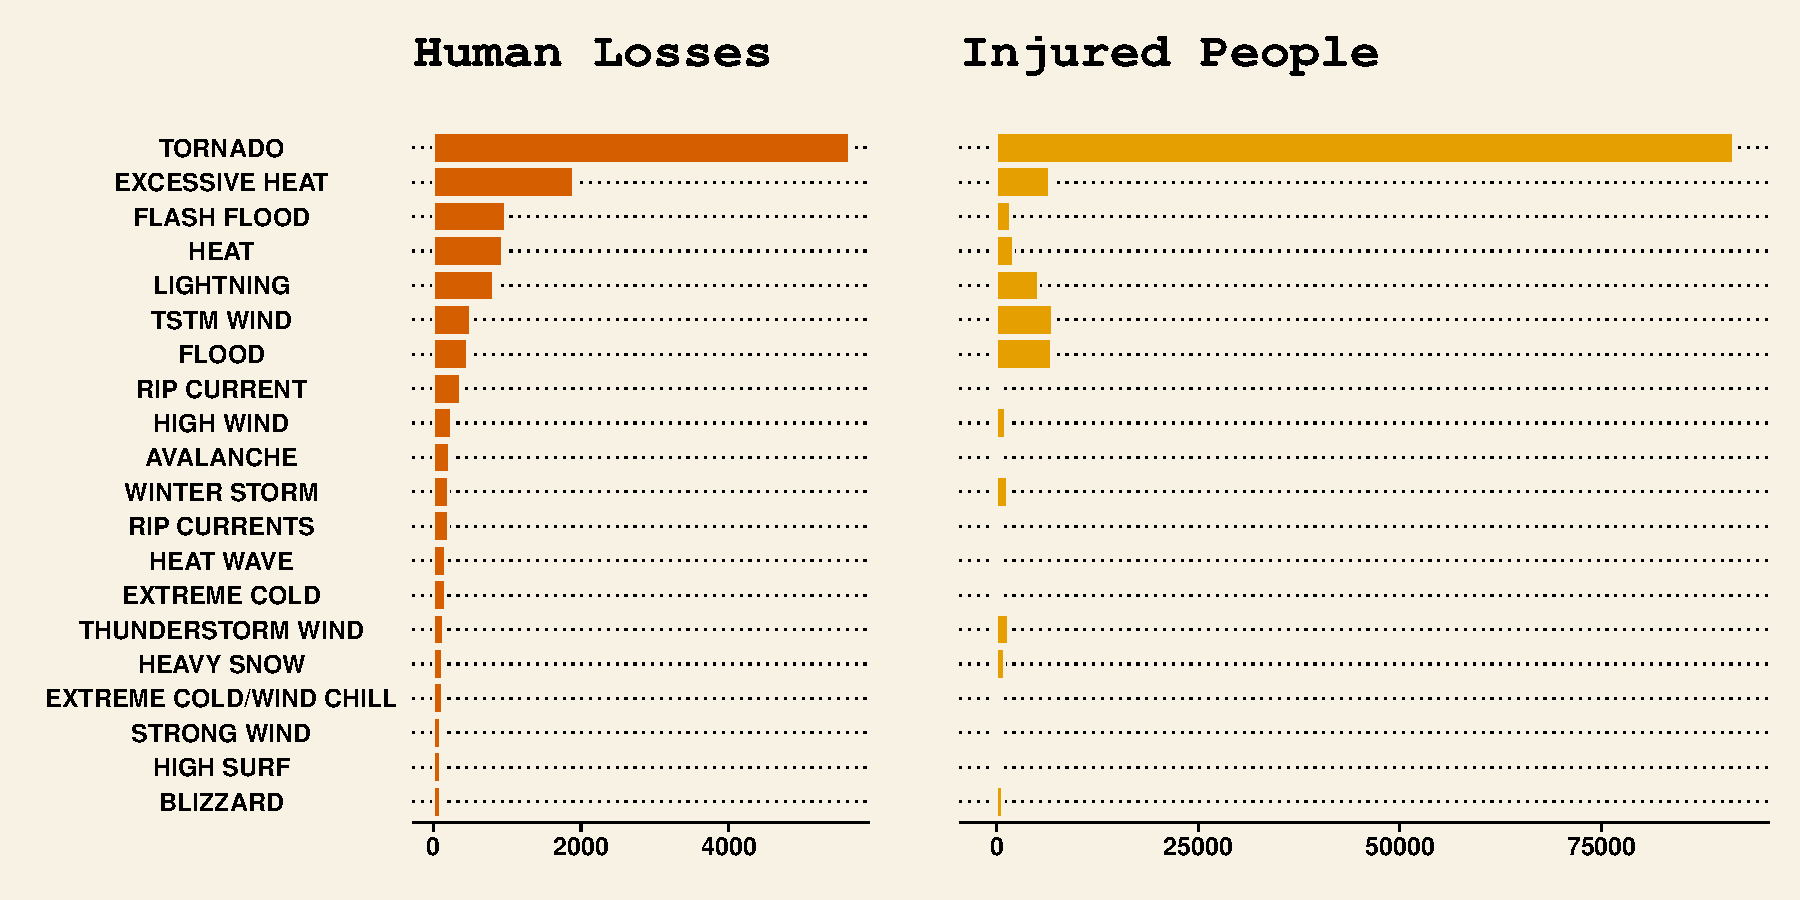
\includegraphics{./proj2_files/figure-latex/ThePlotOne.pdf}
\caption{Events are sorted by the number of fatal cases with a minimum
of 100 fatalities, showing the total number of fatalities and injuries
from 1950 to 2011.}
\end{figure}

The types of events that are most harmful to population health are show
in the above figure and seems that the amount of fatalities and injuries
are related ---as a anecdotical case--- roughly 1:10.

\begin{figure}[htbp]
\centering
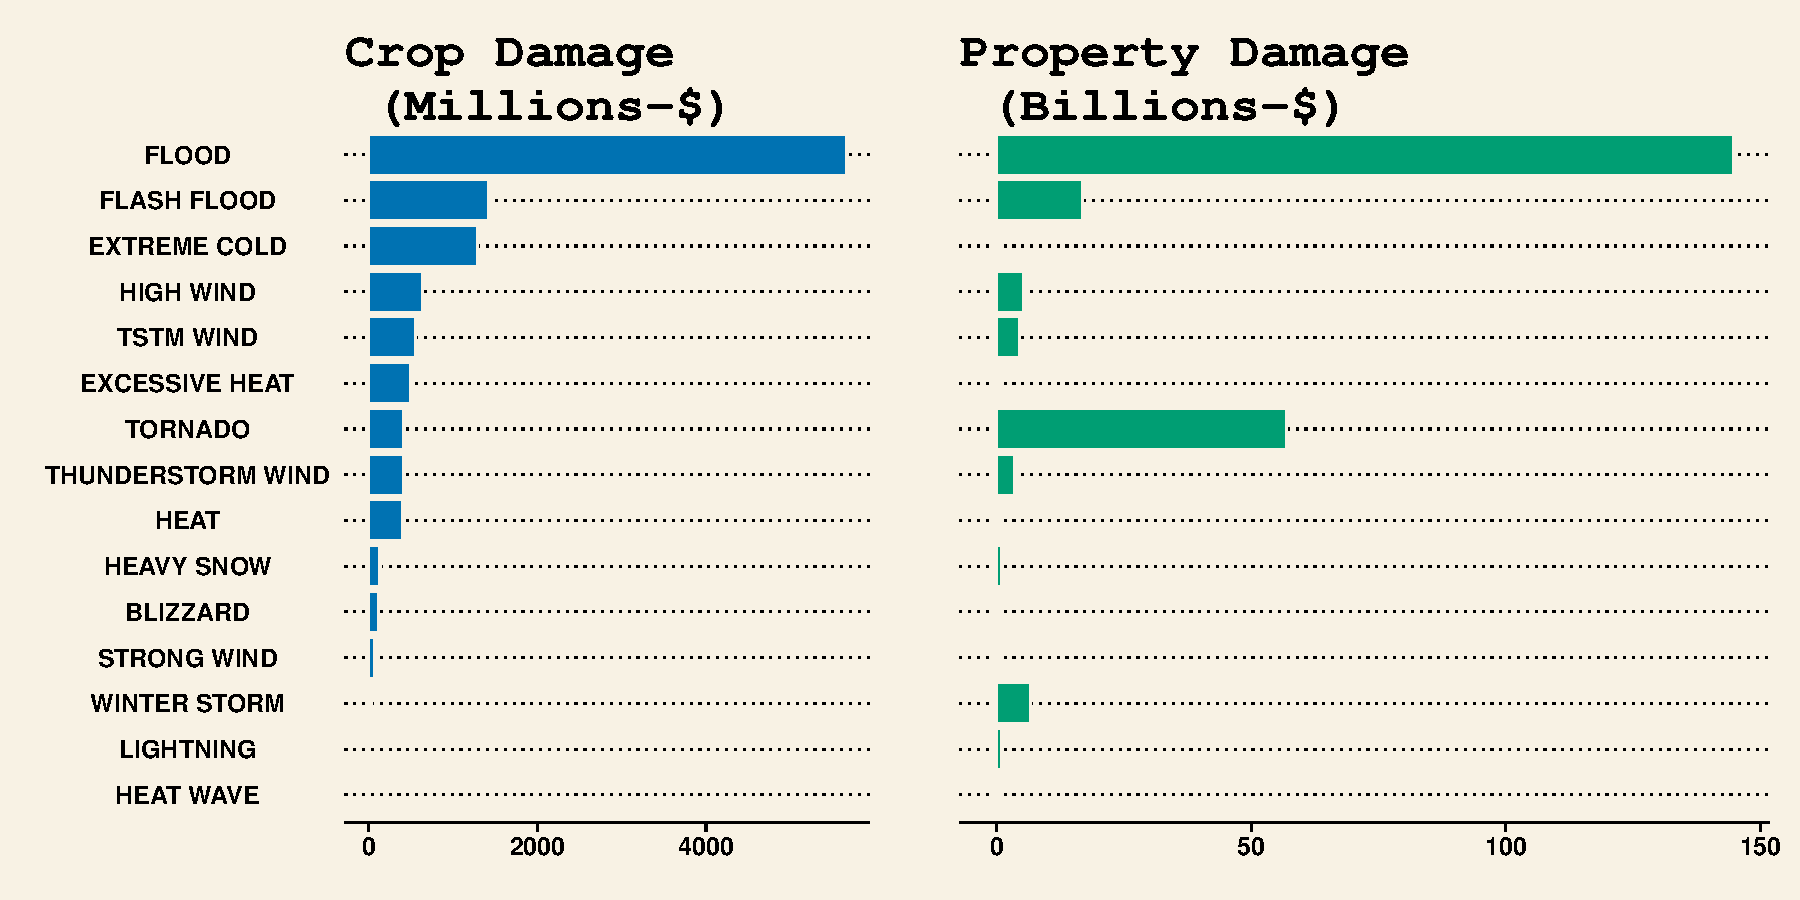
\includegraphics{./proj2_files/figure-latex/ThePlotTwo.pdf}
\caption{Events are sorted by the \$ (million or billion) amount of
damages in crops, with a minimum of one million dollars, showing the
total sum of damage in properties and crops, from 1950 to 2011.}
\end{figure}

The last figure shows the events with the greatest economic consequences
where floods are clearly the most devastating of all events both the
damage they cause to crops and properties

\newpage

\section{Works cited \label{references}}\label{works-cited}

\tiny{ (ACM citation style)} \normalsize
\setlength{\parindent}{-0.40cm} \indent

{[}1{]}CODEBOOK. NATIONAL WEATHER SERVICE INSTRUCTION 10-1605: 2007.
\emph{\url{http://www.ncdc.noaa.gov/stormevents/pd01016005curr.pdf}}.
Accessed: 2014-07-10.

{[}2{]}Multiple Graphs On One Page (ggplot2). FUNCTION CODE OF
MULTIPLOT: 2014.
\emph{\url{http://www.cookbook-r.com/Graphs/Multiple_graphs_on_one_page_(ggplot2)/}}.
Accessed: 2014-07-17.

{[}3{]}Severe Weather Data: 2012.
\emph{\url{http://www.ncdc.noaa.gov/data-access/severe-weather}}.
Accessed: 2014-07-15.

{[}4{]}Storm data for peer assessment 2 - Course: Reproducible Research.
(restricted access, only for COURSERA students): 2014.
\emph{\url{https://class.coursera.org/repdata-004/human_grading/view/courses/972143/assessments/4/submissions}}.
Accessed: 2014-07-10.

{[}5{]}Storm database.: 2012.
\emph{\url{https://d396qusza40orc.cloudfront.net/repdata\%2Fdata\%2FStormData.csv.bz2}}.
Accessed: 2014-07-10.

\newpage

\hyperdef{}{appendix-a}{\section{Appendix A}\label{appendix-a}}

The code that is reproduced below should fully play the manipulation of
data, calculations and presentation of the table and the two images used
in this report. The code is not intended neither to be nice nor
efficient, just get the desired results by giving answer the following
two questions; across the United States, which types of events are most
harmful with respect to population health, and which have the greatest
economic consequences.

\begin{Shaded}
\begin{Highlighting}[]
\CommentTok{# the full listing R code }
\end{Highlighting}
\end{Shaded}

\begin{Shaded}
\begin{Highlighting}[]
\CommentTok{# Getting & loading the data}
\CommentTok{# get the actual working directory}
\NormalTok{curdir <-}\StringTok{ }\KeywordTok{getwd}\NormalTok{()}

\CommentTok{# set the pointer to the working directory where the original }
\CommentTok{# dataset is allocated. Change it to fit your particular setting}
\NormalTok{workingdirectory <-}\StringTok{ "D:/Cursos/Hopkin/5-Reproducible Research/Project 2"}

\CommentTok{# set the new working directory}
\KeywordTok{setwd}\NormalTok{(workingdirectory)}

\CommentTok{# loading the dataset that is already in the working diractory }
\NormalTok{myNOAA <-}\StringTok{ }\KeywordTok{read.csv}\NormalTok{(}\StringTok{"./repdatadataStormData.csv.bz2"}\NormalTok{)}

\CommentTok{# add a variable with only the year, becuase maybe we need it}
\NormalTok{myNOAA <-}\StringTok{ }\KeywordTok{subset}\NormalTok{(myNOAA, }\DataTypeTok{select=}\KeywordTok{c}\NormalTok{(}\StringTok{"BGN_DATE"}\NormalTok{,}
                                  \StringTok{"EVTYPE"}\NormalTok{,}
                                  \StringTok{"FATALITIES"}\NormalTok{,}
                                  \StringTok{"INJURIES"}\NormalTok{,}
                                  \StringTok{"PROPDMG"}\NormalTok{,}
                                  \StringTok{"PROPDMGEXP"}\NormalTok{,}
                                  \StringTok{"CROPDMG"}\NormalTok{,}
                                  \StringTok{"CROPDMGEXP"}\NormalTok{))}
\end{Highlighting}
\end{Shaded}

\begin{Shaded}
\begin{Highlighting}[]
\NormalTok{####################}
\NormalTok{##### function multiplot}
\NormalTok{####################}

\CommentTok{# Multiple plot function}
\CommentTok{# from http://www.cookbook-r.com/Graphs/Multiple_graphs_on_one_page_%28ggplot2%29/}
\CommentTok{#}
\CommentTok{# ggplot objects can be passed in ..., or to plotlist (as a list of ggplot objects)}
\CommentTok{# - cols:   Number of columns in layout}
\CommentTok{# - layout: A matrix specifying the layout. If present, 'cols' is ignored.}
\CommentTok{#}
\CommentTok{# If the layout is something like matrix(c(1,2,3,3), nrow=2, byrow=TRUE),}
\CommentTok{# then plot 1 will go in the upper left, 2 will go in the upper right, and}
\CommentTok{# 3 will go all the way across the bottom.}
\CommentTok{#}
\CommentTok{#}
\NormalTok{multiplot <-}\StringTok{ }\NormalTok{function(..., }\DataTypeTok{plotlist=}\OtherTok{NULL}\NormalTok{, file, }\DataTypeTok{cols=}\DecValTok{1}\NormalTok{, }\DataTypeTok{layout=}\OtherTok{NULL}\NormalTok{) \{}
  \KeywordTok{require}\NormalTok{(grid)}
  
  \CommentTok{# Make a list from the ... arguments and plotlist}
  \NormalTok{plots <-}\StringTok{ }\KeywordTok{c}\NormalTok{(}\KeywordTok{list}\NormalTok{(...), plotlist)}
  
  \NormalTok{numPlots =}\StringTok{ }\KeywordTok{length}\NormalTok{(plots)}
  
  \CommentTok{# If layout is NULL, then use 'cols' to determine layout}
  \NormalTok{if (}\KeywordTok{is.null}\NormalTok{(layout)) \{}
    \CommentTok{# Make the panel}
    \CommentTok{# ncol: Number of columns of plots}
    \CommentTok{# nrow: Number of rows needed, calculated from # of cols}
    \NormalTok{layout <-}\StringTok{ }\KeywordTok{matrix}\NormalTok{(}\KeywordTok{seq}\NormalTok{(}\DecValTok{1}\NormalTok{, cols *}\StringTok{ }\KeywordTok{ceiling}\NormalTok{(numPlots/cols)),}
                     \DataTypeTok{ncol =} \NormalTok{cols, }\DataTypeTok{nrow =} \KeywordTok{ceiling}\NormalTok{(numPlots/cols))}
  \NormalTok{\}}
  
  \NormalTok{if (numPlots==}\DecValTok{1}\NormalTok{) \{}
    \KeywordTok{print}\NormalTok{(plots[[}\DecValTok{1}\NormalTok{]])}
    
  \NormalTok{\} else \{}
    \CommentTok{# Set up the page}
    \KeywordTok{grid.newpage}\NormalTok{()}
    \KeywordTok{pushViewport}\NormalTok{(}\KeywordTok{viewport}\NormalTok{(}\DataTypeTok{layout =} \KeywordTok{grid.layout}\NormalTok{(}\KeywordTok{nrow}\NormalTok{(layout), }\KeywordTok{ncol}\NormalTok{(layout))))}
    
    \CommentTok{# Make each plot, in the correct location}
    \NormalTok{for (i in }\DecValTok{1}\NormalTok{:numPlots) \{}
      \CommentTok{# Get the i,j matrix positions of the regions that contain this subplot}
      \NormalTok{matchidx <-}\StringTok{ }\KeywordTok{as.data.frame}\NormalTok{(}\KeywordTok{which}\NormalTok{(layout ==}\StringTok{ }\NormalTok{i, }\DataTypeTok{arr.ind =} \OtherTok{TRUE}\NormalTok{))}
      
      \KeywordTok{print}\NormalTok{(plots[[i]], }\DataTypeTok{vp =} \KeywordTok{viewport}\NormalTok{(}\DataTypeTok{layout.pos.row =} \NormalTok{matchidx$row,}
                                      \DataTypeTok{layout.pos.col =} \NormalTok{matchidx$col))}
    \NormalTok{\}}
  \NormalTok{\}}
\NormalTok{\}}

\NormalTok{####################}
\NormalTok{##### End of function multiplot}
\NormalTok{####################}
\end{Highlighting}
\end{Shaded}

\begin{Shaded}
\begin{Highlighting}[]
\CommentTok{# attach the dataset so we don't need to write large names}
\KeywordTok{attach}\NormalTok{(myNOAA)}

\CommentTok{# add a variable to the dataset with only the year}
\NormalTok{myNOAA$BGN_YEAR <-}\StringTok{ }\KeywordTok{format}\NormalTok{(}\KeywordTok{as.Date}\NormalTok{(BGN_DATE, }\DataTypeTok{format =} \StringTok{"%m/%d/%Y"}\NormalTok{), }\StringTok{"%Y"}\NormalTok{)}

\CommentTok{# create a new variable same as PROPDMGEXP}
\NormalTok{myNOAA$PROPEXP <-}\StringTok{ }\NormalTok{PROPDMGEXP}

\CommentTok{# actual levels of PROPDMGEXP =}
\CommentTok{# ""  "-" "?" "+" "0" "1" "2" "3" "4" "5" "6" "7" "8" "B" "h" "H" "K" "m" "M"}

\CommentTok{# but we want to be =}
\NormalTok{niveles <-}\KeywordTok{c}\NormalTok{(}\StringTok{"0"}\NormalTok{, }\StringTok{"0"}\NormalTok{, }\StringTok{"0"}\NormalTok{, }\StringTok{"0"}\NormalTok{, }
            \StringTok{"1"}\NormalTok{, }\StringTok{"10"}\NormalTok{, }\StringTok{"100"}\NormalTok{, }\StringTok{"1000"}\NormalTok{, }\StringTok{"10000"}\NormalTok{, }
            \StringTok{"100000"}\NormalTok{, }\StringTok{"1000000"}\NormalTok{, }\StringTok{"10000000"}\NormalTok{, }\StringTok{"100000000"}\NormalTok{,}
            \StringTok{"1000000000"}\NormalTok{, }\StringTok{"100"}\NormalTok{, }\StringTok{"100"}\NormalTok{, }\StringTok{"1000"}\NormalTok{, }\StringTok{"1000000"}\NormalTok{, }\StringTok{"1000000"}\NormalTok{)}

\CommentTok{# so, do it}
\KeywordTok{levels}\NormalTok{(myNOAA$PROPEXP) <-}\StringTok{ }\NormalTok{niveles}

\CommentTok{# change from factor to char ...}
\NormalTok{myNOAA$PROPEXP <-}\StringTok{ }\KeywordTok{as.character}\NormalTok{(myNOAA$PROPEXP)}

\CommentTok{# change from char to numeric}
\NormalTok{myNOAA$PROPEXP <-}\StringTok{ }\KeywordTok{as.numeric}\NormalTok{(myNOAA$PROPEXP)}

\CommentTok{# calculate the value in billions of dollars and save it as a new variable}
\NormalTok{million=}\KeywordTok{as.numeric}\NormalTok{(}\DecValTok{1000000}\NormalTok{)}
\NormalTok{billion=}\KeywordTok{as.numeric}\NormalTok{(}\DecValTok{1000000000}\NormalTok{)}


\NormalTok{myNOAA$PROP <-}\StringTok{ }\NormalTok{PROPDMG *}\StringTok{ }\NormalTok{myNOAA$PROPEXP}
\NormalTok{myNOAA$PROP <-}\StringTok{ }\NormalTok{myNOAA$PROP/billion}

\CommentTok{#}
\CommentTok{# now, we do the same as the above, but now for CROPDMGEXP}
\CommentTok{#}
\NormalTok{myNOAA$CROPEXP <-}\StringTok{ }\NormalTok{CROPDMGEXP}

\CommentTok{# actual levels of PROPDMGEXP =}
\CommentTok{# ""  "?" "0" "2" "B" "k" "K" "m" "M"}
\CommentTok{# but we want  =}
\NormalTok{niveles <-}\KeywordTok{c}\NormalTok{(}\StringTok{"0"}\NormalTok{, }\StringTok{"0"}\NormalTok{, }
            \StringTok{"1"}\NormalTok{, }\StringTok{"100"}\NormalTok{, }
            \StringTok{"1000000000"}\NormalTok{, }\StringTok{"1000"}\NormalTok{, }\StringTok{"1000"}\NormalTok{,}\StringTok{"1000000"}\NormalTok{,}\StringTok{"1000000"}\NormalTok{)}

\CommentTok{# so, do it, as we did it above ...}
\KeywordTok{levels}\NormalTok{(myNOAA$CROPEXP) <-}\StringTok{ }\NormalTok{niveles}
\NormalTok{myNOAA$CROPEXP <-}\StringTok{ }\KeywordTok{as.character}\NormalTok{(myNOAA$CROPEXP)}
\NormalTok{myNOAA$CROPEXP <-}\StringTok{ }\KeywordTok{as.numeric}\NormalTok{(myNOAA$CROPEXP)}

\CommentTok{# calculate the value in millions of dollars and save it as a new variable}
\NormalTok{myNOAA$CROP <-}\StringTok{ }\NormalTok{CROPDMG *}\StringTok{ }\NormalTok{myNOAA$CROPEXP}
\NormalTok{myNOAA$CROP <-}\StringTok{ }\NormalTok{myNOAA$CROP /}\StringTok{ }\NormalTok{million}
\CommentTok{# no more attachment}
\KeywordTok{detach}\NormalTok{(myNOAA)}
\end{Highlighting}
\end{Shaded}

\begin{Shaded}
\begin{Highlighting}[]
\CommentTok{# goupe the data by EVTYPE summming the fatal cases}
\NormalTok{fatalEvent <-}\StringTok{ }\KeywordTok{aggregate}\NormalTok{(FATALITIES ~}\StringTok{ }\NormalTok{EVTYPE, myNOAA, sum)}

\CommentTok{# goupe the data by EVTYPE summming the injuried cases}
\NormalTok{injurEvent <-}\StringTok{ }\KeywordTok{aggregate}\NormalTok{(INJURIES ~}\StringTok{ }\NormalTok{EVTYPE, myNOAA, sum)}

\CommentTok{# merge those two data frames into health one}
\NormalTok{healthEvent <-}\StringTok{ }\KeywordTok{merge}\NormalTok{(fatalEvent, injurEvent, }\DataTypeTok{by=}\StringTok{"EVTYPE"}\NormalTok{, }\DataTypeTok{sort =} \OtherTok{FALSE}\NormalTok{)}

\CommentTok{# goupe the data by EVTYPE summming the property cases}
\NormalTok{propEvent <-}\StringTok{ }\KeywordTok{aggregate}\NormalTok{(PROP ~}\StringTok{ }\NormalTok{EVTYPE, myNOAA, sum)}

\CommentTok{# goupe the data by EVTYPE summming the crop cases}
\NormalTok{cropEvent <-}\StringTok{ }\KeywordTok{aggregate}\NormalTok{(CROP ~}\StringTok{ }\NormalTok{EVTYPE, myNOAA, sum)}

\CommentTok{# merge those two data frames into economic one}
\NormalTok{economicEvent <-}\StringTok{ }\KeywordTok{merge}\NormalTok{(propEvent, cropEvent, }\DataTypeTok{by=}\StringTok{"EVTYPE"}\NormalTok{, }\DataTypeTok{sort =} \OtherTok{FALSE}\NormalTok{)}

\CommentTok{# merge health and economic data frames into a fulldata one}
\NormalTok{FullData <-}\StringTok{ }\KeywordTok{merge}\NormalTok{(healthEvent, economicEvent, }\DataTypeTok{by=}\StringTok{"EVTYPE"}\NormalTok{, }\DataTypeTok{sort =} \OtherTok{FALSE}\NormalTok{)}

\CommentTok{# save the data in the local disc}
\KeywordTok{write.table}\NormalTok{(myNOAA, }\StringTok{"./myNOAA.txt"}\NormalTok{, }\DataTypeTok{sep=}\StringTok{"}\CharTok{\textbackslash{}t}\StringTok{"}\NormalTok{)}
\KeywordTok{write.table}\NormalTok{(FullData, }\StringTok{"./FullData.txt"}\NormalTok{, }\DataTypeTok{sep=}\StringTok{"}\CharTok{\textbackslash{}t}\StringTok{"}\NormalTok{)}
\end{Highlighting}
\end{Shaded}

\begin{Shaded}
\begin{Highlighting}[]
\CommentTok{# Load the required libraries to plot and make the latex/HTML table}
\KeywordTok{require}\NormalTok{(ggthemes)}
\KeywordTok{require}\NormalTok{(grid)}
\KeywordTok{require}\NormalTok{(gtable)}
\KeywordTok{require}\NormalTok{(xtable)}

\CommentTok{# and the libraries to format the outputs from this own Rmarkdown file }
\CommentTok{# to incorporate the table printout as a latex commands to be printed as }
\CommentTok{# part of this file aoutput.}
\CommentTok{# Note, that the output could be also as a HTML format.}
\KeywordTok{require}\NormalTok{(plyr)}
\KeywordTok{require}\NormalTok{(knitr)}

\CommentTok{# in order to show data in table and plots, we choose the minimum cases }
\CommentTok{# for the healt affected as the sum of fatal and injuries cases.}
\CommentTok{# for this analysis the value will be 100 persons as minimum.}

\NormalTok{myDataEvent <-}\StringTok{ }\NormalTok{FullData}
\NormalTok{MinimumPeopleAfected <-}\StringTok{ }\DecValTok{100}
\NormalTok{myDataEvent <-}\StringTok{ }\NormalTok{myDataEvent[myDataEvent$FATALITIES >}\StringTok{ }\NormalTok{MinimumPeopleAfected, ]}

\NormalTok{myDataEvent <-}\StringTok{ }\KeywordTok{droplevels}\NormalTok{(myDataEvent)}

\CommentTok{# prepare to table}
\KeywordTok{names}\NormalTok{(myDataEvent) <-}\StringTok{ }\KeywordTok{c}\NormalTok{(}\StringTok{"Event"}\NormalTok{,}\StringTok{"Fatalities"}\NormalTok{, }\StringTok{"Injuries"}\NormalTok{, }\StringTok{"Property(B$)"}\NormalTok{, }\StringTok{"Crop(M$)"}\NormalTok{)}

\CommentTok{# re-order the dataframe to be tabulated and convert num into integers}
\CommentTok{# to show them in table}

\NormalTok{tmp <-}\StringTok{ }\KeywordTok{arrange}\NormalTok{(myDataEvent, -Fatalities)}
\NormalTok{tmp$Fatalities <-}\StringTok{ }\KeywordTok{as.integer}\NormalTok{(tmp$Fatalities)}
\NormalTok{tmp$Injuries <-}\StringTok{ }\KeywordTok{as.integer}\NormalTok{(tmp$Injuries)}

\NormalTok{myCaption =}\StringTok{ 'Sed nec mi tincidunt, feugiat arcu ac, malesuada mauris. Suspendisse et scelerisque erat. Phasellus vitae risus at justo tincidunt posuere. Fusce eget nisi a justo ullamcorper condimentum.'}

\NormalTok{tmpTABLE <-}\StringTok{ }\NormalTok{tmp}

\NormalTok{myLatexTable <-}\StringTok{ }\KeywordTok{print}\NormalTok{(}\KeywordTok{xtable}\NormalTok{(tmpTABLE, }\DataTypeTok{caption=}\NormalTok{myCaption),}
                      \DataTypeTok{type=}\StringTok{'latex'}\NormalTok{, }
                      \DataTypeTok{comment =} \OtherTok{FALSE}\NormalTok{)}
\end{Highlighting}
\end{Shaded}

\begin{Shaded}
\begin{Highlighting}[]
\CommentTok{# Load the required libraries to plot and make the latex table}
\KeywordTok{require}\NormalTok{(ggthemes)}
\KeywordTok{require}\NormalTok{(grid)}
\KeywordTok{require}\NormalTok{(gtable)}
\KeywordTok{require}\NormalTok{(xtable)}

\CommentTok{# and the libraries to format the outputs from this own Rmarkdown file }
\CommentTok{# to incorporate the table printout as a latex commands to be printed as }
\CommentTok{# part of this file aoutput.}
\CommentTok{# Note, that the output could be also as a HTML format.}
\KeywordTok{require}\NormalTok{(plyr)}
\KeywordTok{require}\NormalTok{(knitr)}

\CommentTok{# in order to show data in table and plots, we choose the minimum cases }
\CommentTok{# for the healt affected as the sum of fatal and injuries cases.}
\CommentTok{# for this analysis the value will be 100 persons as minimum.}

\NormalTok{myDataEvent <-}\StringTok{ }\NormalTok{FullData}
\NormalTok{MinimumPeopleAfected <-}\StringTok{ }\DecValTok{100}
\NormalTok{myDataEvent <-}\StringTok{ }\NormalTok{myDataEvent[myDataEvent$FATALITIES >}\StringTok{ }\NormalTok{MinimumPeopleAfected, ]}

\NormalTok{myDataEvent <-}\StringTok{ }\KeywordTok{droplevels}\NormalTok{(myDataEvent)}

\CommentTok{# prepare to table}
\KeywordTok{names}\NormalTok{(myDataEvent) <-}\StringTok{ }\KeywordTok{c}\NormalTok{(}\StringTok{"Event"}\NormalTok{,}
                        \StringTok{"Fatalities"}\NormalTok{, }
                        \StringTok{"Injuries"}\NormalTok{, }
                        \StringTok{"Property(B$)"}\NormalTok{, }
                        \StringTok{"Crop(M$)"}\NormalTok{)}

\CommentTok{# re-order the dataframe to be tabulated and convert num into integers}
\CommentTok{# to show them in table}

\NormalTok{tmp <-}\StringTok{ }\KeywordTok{arrange}\NormalTok{(myDataEvent, -Fatalities)}
\NormalTok{tmp$Fatalities <-}\StringTok{ }\KeywordTok{as.integer}\NormalTok{(tmp$Fatalities)}
\NormalTok{tmp$Injuries <-}\StringTok{ }\KeywordTok{as.integer}\NormalTok{(tmp$Injuries)}

\CommentTok{# to reproduce enterely the long sentence for the caption let's do a trick ...}
\NormalTok{myCaption <-}\StringTok{ }\KeywordTok{paste}\NormalTok{(}\StringTok{"Rearrangement, respect to the type of event,"}\NormalTok{,}
                   \StringTok{"of the four values we are interested; cases of"}\NormalTok{,}
                   \StringTok{"fatalities and injuries, and also, damages"}\NormalTok{,}
                   \StringTok{"to properties and crop."}\NormalTok{,  }\DataTypeTok{sep =} \StringTok{" "}\NormalTok{)}
                   
\NormalTok{tmpTABLE <-}\StringTok{ }\NormalTok{tmp}

\NormalTok{myLatexTable <-}\StringTok{ }\KeywordTok{print}\NormalTok{(}\KeywordTok{xtable}\NormalTok{(tmpTABLE, }\DataTypeTok{caption=}\NormalTok{myCaption),}
                      \DataTypeTok{type=}\StringTok{'latex'}\NormalTok{, }
                      \DataTypeTok{comment =} \OtherTok{FALSE}\NormalTok{)}
\end{Highlighting}
\end{Shaded}

\begin{Shaded}
\begin{Highlighting}[]
\CommentTok{# Load the required libraries to plot and make the latex/HTML table}
\KeywordTok{require}\NormalTok{(ggthemes)}
\KeywordTok{require}\NormalTok{(grid)}
\KeywordTok{require}\NormalTok{(gtable)}

\CommentTok{# construct a friendly palette to Colorblind People as recommended by}
\CommentTok{# Color Universal Design (CUD), and add the the default gray from ggplot}
\CommentTok{# and the salmon from Wall Street Journal theme  background. }
\CommentTok{# We could also add Black = "#000000", but better not to use it.}

\NormalTok{Gray =}\StringTok{ "#999999"} 
\NormalTok{Orange =}\StringTok{ "#E69F00"}
\NormalTok{SkyBlue =}\StringTok{ "#56B4E9"}
\NormalTok{BluishGreen =}\StringTok{ "#009E73"}
\NormalTok{Yellow =}\StringTok{ "#F0E442"}
\NormalTok{Blue =}\StringTok{ "#0072B2"}
\NormalTok{Vermillon =}\StringTok{ "#D55E00"}
\NormalTok{RedddishPurple =}\StringTok{ "#CC79A7"}
\NormalTok{GrayGGplot =}\StringTok{"#E5E5E5"}
\NormalTok{SalmonWSJ =}\StringTok{ "#F8F2E4"}

\NormalTok{cbPalette <-}\StringTok{ }\KeywordTok{c}\NormalTok{(Gray,}
               \NormalTok{Orange,}
               \NormalTok{SkyBlue,}
               \NormalTok{BluishGreen,}
               \NormalTok{Yellow,}
               \NormalTok{Blue,}
               \NormalTok{Vermillon,}
               \NormalTok{RedddishPurple,}
               \NormalTok{GrayGGplot,}
               \NormalTok{SalmonWSJ)}
\end{Highlighting}
\end{Shaded}

\begin{Shaded}
\begin{Highlighting}[]
\NormalTok{p1 <-}\StringTok{ }\KeywordTok{ggplot}\NormalTok{(tmp, }\DataTypeTok{height=}\DecValTok{480}\NormalTok{, }\DataTypeTok{width=}\DecValTok{480}\NormalTok{) +}\StringTok{ }
\StringTok{  }\KeywordTok{scale_fill_manual}\NormalTok{(}\DataTypeTok{values=}\NormalTok{cbPalette[}\DecValTok{7}\NormalTok{]) +}
\StringTok{  }\KeywordTok{scale_colour_manual}\NormalTok{(}\DataTypeTok{values=}\NormalTok{cbPalette[}\DecValTok{10}\NormalTok{]) +}
\StringTok{  }\KeywordTok{aes}\NormalTok{(}\DataTypeTok{x=}\NormalTok{Event, }\DataTypeTok{y=} \NormalTok{Fatalities, }\DataTypeTok{fill=} \StringTok{"manual"}\NormalTok{, }\DataTypeTok{colour =} \StringTok{"manual"}\NormalTok{) +}
\StringTok{  }\KeywordTok{geom_bar}\NormalTok{(}\DataTypeTok{stat=}\StringTok{"identity"}\NormalTok{) +}
\StringTok{  }\KeywordTok{coord_flip}\NormalTok{() +}\StringTok{ }
\StringTok{  }\KeywordTok{theme}\NormalTok{(}\DataTypeTok{legend.position=}\StringTok{"none"}\NormalTok{) +}\StringTok{ }
\StringTok{  }\KeywordTok{xlab}\NormalTok{(}\StringTok{""}\NormalTok{) +}\StringTok{ }
\StringTok{  }\KeywordTok{ylab}\NormalTok{(}\StringTok{""}\NormalTok{) +}\StringTok{ }
\StringTok{  }\KeywordTok{ggtitle}\NormalTok{(}\KeywordTok{paste}\NormalTok{(}\StringTok{"Human Losses"}\NormalTok{,}\StringTok{"}\CharTok{\textbackslash{}n}\StringTok{"}\NormalTok{)) +}
\StringTok{  }\KeywordTok{theme}\NormalTok{(}\DataTypeTok{legend.position=}\StringTok{"none"}\NormalTok{) +}
\StringTok{  }\KeywordTok{theme}\NormalTok{(}\DataTypeTok{axis.text.y=}\KeywordTok{element_blank}\NormalTok{())}

\CommentTok{# give a look&fell like The Wall Street Journal use ... }
\NormalTok{g1 <-}\StringTok{ }\NormalTok{p1 +}\StringTok{ }
\StringTok{  }\KeywordTok{theme_wsj}\NormalTok{() +}
\StringTok{  }\KeywordTok{theme}\NormalTok{(}\DataTypeTok{legend.position=}\StringTok{"none"}\NormalTok{)}

\CommentTok{# save the plot }
\KeywordTok{png}\NormalTok{(}\DataTypeTok{file =} \StringTok{"./myproject2_files/figure-latex/plot1.png"}\NormalTok{, }
    \DataTypeTok{width =} \DecValTok{480}\NormalTok{, }
    \DataTypeTok{height =} \DecValTok{480}\NormalTok{, }
    \DataTypeTok{units =} \StringTok{"px"}\NormalTok{, }
    \DataTypeTok{pointsize =} \DecValTok{12}\NormalTok{,}
    \DataTypeTok{bg =} \StringTok{"transparent"}\NormalTok{)}

\KeywordTok{plot}\NormalTok{(g1)}

\KeywordTok{dev.off}\NormalTok{() ->}\StringTok{ }\NormalTok{trashcan}
\end{Highlighting}
\end{Shaded}

\begin{Shaded}
\begin{Highlighting}[]
\NormalTok{p2 <-}\StringTok{ }\KeywordTok{ggplot}\NormalTok{(tmp, }\DataTypeTok{height=}\DecValTok{480}\NormalTok{, }\DataTypeTok{width=}\DecValTok{480}\NormalTok{) +}\StringTok{ }
\StringTok{  }\KeywordTok{scale_fill_manual}\NormalTok{(}\DataTypeTok{values=}\NormalTok{cbPalette[}\DecValTok{2}\NormalTok{]) +}
\StringTok{  }\KeywordTok{scale_colour_manual}\NormalTok{(}\DataTypeTok{values=}\NormalTok{cbPalette[}\DecValTok{10}\NormalTok{]) +}
\StringTok{  }\KeywordTok{aes}\NormalTok{(}\DataTypeTok{x=}\NormalTok{Event, }\DataTypeTok{y=} \NormalTok{Injuries, }\DataTypeTok{fill=} \StringTok{"manual"}\NormalTok{, }\DataTypeTok{colour =} \StringTok{"manual"}\NormalTok{) +}
\StringTok{  }\KeywordTok{geom_bar}\NormalTok{(}\DataTypeTok{stat=}\StringTok{"identity"}\NormalTok{) +}
\StringTok{  }\KeywordTok{coord_flip}\NormalTok{() +}\StringTok{ }
\StringTok{  }\KeywordTok{theme}\NormalTok{(}\DataTypeTok{legend.position=}\StringTok{"none"}\NormalTok{) +}\StringTok{ }
\StringTok{  }\KeywordTok{xlab}\NormalTok{(}\StringTok{""}\NormalTok{) +}\StringTok{ }
\StringTok{  }\KeywordTok{ylab}\NormalTok{(}\StringTok{""}\NormalTok{) +}\StringTok{ }
\StringTok{  }\KeywordTok{ggtitle}\NormalTok{(}\KeywordTok{paste}\NormalTok{(}\StringTok{"Injured People"}\NormalTok{,}\StringTok{"}\CharTok{\textbackslash{}n}\StringTok{"}\NormalTok{)) +}
\StringTok{  }\KeywordTok{theme}\NormalTok{(}\DataTypeTok{legend.position=}\StringTok{"none"}\NormalTok{)}

\CommentTok{# give a look&fell like The Wall Street Journal use ... }
\NormalTok{g2 <-}\StringTok{ }\NormalTok{p2 +}\StringTok{ }
\StringTok{  }\KeywordTok{theme_wsj}\NormalTok{() +}
\StringTok{  }\KeywordTok{theme}\NormalTok{(}\DataTypeTok{legend.position=}\StringTok{"none"}\NormalTok{, }\DataTypeTok{axis.text.y=}\KeywordTok{element_blank}\NormalTok{())}

\CommentTok{# save the plot }
\KeywordTok{png}\NormalTok{(}\DataTypeTok{file =} \StringTok{"./myproject2_files/figure-latex/plot2.png"}\NormalTok{, }
    \DataTypeTok{width =} \DecValTok{480}\NormalTok{, }
    \DataTypeTok{height =} \DecValTok{480}\NormalTok{, }
    \DataTypeTok{units =} \StringTok{"px"}\NormalTok{, }
    \DataTypeTok{pointsize =} \DecValTok{12}\NormalTok{,}
    \DataTypeTok{bg =} \StringTok{"transparent"}\NormalTok{)}

\KeywordTok{plot}\NormalTok{(g2)}

\KeywordTok{dev.off}\NormalTok{() ->}\StringTok{ }\NormalTok{trashcan}
\end{Highlighting}
\end{Shaded}

\begin{Shaded}
\begin{Highlighting}[]
\CommentTok{# show the plot of injured and losses human }
\CommentTok{# as figure 1.}
\CommentTok{# Note, the figure caption is in the heading of the correspondent chunk}
\KeywordTok{multiplot}\NormalTok{(g1, g2, }\DataTypeTok{cols=}\DecValTok{2}\NormalTok{)}

\CommentTok{# save it}
\KeywordTok{png}\NormalTok{(}\DataTypeTok{file =} \StringTok{"./myproject2_files/figure-latex/PlotOne.png"}\NormalTok{, }
    \DataTypeTok{width =} \DecValTok{960}\NormalTok{, }
    \DataTypeTok{height =} \DecValTok{480}\NormalTok{, }
    \DataTypeTok{units =} \StringTok{"px"}\NormalTok{, }
    \DataTypeTok{pointsize =} \DecValTok{12}\NormalTok{,}
    \DataTypeTok{bg =} \StringTok{"transparent"}\NormalTok{)}

\KeywordTok{multiplot}\NormalTok{(g1, g2, }\DataTypeTok{cols=}\DecValTok{2}\NormalTok{)}

\KeywordTok{dev.off}\NormalTok{() ->}\StringTok{ }\NormalTok{trashcan}
\end{Highlighting}
\end{Shaded}

\begin{Shaded}
\begin{Highlighting}[]
\NormalTok{MinimumCropDamage <-}\StringTok{ }\DecValTok{1}
\NormalTok{tmp <-}\StringTok{ }\NormalTok{myDataEvent[tmp$Crop >}\StringTok{ }\NormalTok{MinimumCropDamage, ]}

\NormalTok{tmp <-}\StringTok{ }\KeywordTok{droplevels}\NormalTok{(tmp)}

\CommentTok{# re-order the data with crop damages}

\KeywordTok{require}\NormalTok{(plyr)}


\NormalTok{tmp$Event <-}\StringTok{ }\KeywordTok{factor}\NormalTok{(tmp$Event,}
                    \DataTypeTok{levels=} \NormalTok{tmp[}\KeywordTok{order}\NormalTok{(tmp$Crop), ]$Event)}

\NormalTok{myorder <-}\StringTok{ }\KeywordTok{levels}\NormalTok{(tmp$Event)}

\NormalTok{tmp$Event <-}\StringTok{ }\KeywordTok{factor}\NormalTok{(tmp$Event, }\DataTypeTok{levels=}\NormalTok{myorder, }\DataTypeTok{ordered=}\OtherTok{TRUE}\NormalTok{)}

\NormalTok{p3 <-}\StringTok{ }\KeywordTok{ggplot}\NormalTok{(tmp, }\DataTypeTok{height=}\DecValTok{480}\NormalTok{, }\DataTypeTok{width=}\DecValTok{480}\NormalTok{) +}\StringTok{ }
\StringTok{  }\KeywordTok{scale_fill_manual}\NormalTok{(}\DataTypeTok{values=}\NormalTok{cbPalette[}\DecValTok{4}\NormalTok{]) +}
\StringTok{  }\KeywordTok{scale_colour_manual}\NormalTok{(}\DataTypeTok{values=}\NormalTok{cbPalette[}\DecValTok{10}\NormalTok{]) +}
\StringTok{  }\KeywordTok{aes}\NormalTok{(}\DataTypeTok{x=}\NormalTok{Event, }\DataTypeTok{y=} \NormalTok{Property, }\DataTypeTok{fill=} \StringTok{"manual"}\NormalTok{, }\DataTypeTok{colour =} \StringTok{"manual"}\NormalTok{) +}
\StringTok{  }\KeywordTok{geom_bar}\NormalTok{(}\DataTypeTok{stat=}\StringTok{"identity"}\NormalTok{) +}
\StringTok{  }\KeywordTok{coord_flip}\NormalTok{() +}\StringTok{ }
\StringTok{  }\KeywordTok{theme}\NormalTok{(}\DataTypeTok{legend.position=}\StringTok{"none"}\NormalTok{) +}\StringTok{ }
\StringTok{  }\KeywordTok{xlab}\NormalTok{(}\StringTok{""}\NormalTok{) +}\StringTok{ }
\StringTok{  }\KeywordTok{ylab}\NormalTok{(}\StringTok{""}\NormalTok{) +}\StringTok{ }
\StringTok{  }\KeywordTok{ggtitle}\NormalTok{(}\KeywordTok{paste}\NormalTok{(}\StringTok{"Property Damage}\CharTok{\textbackslash{}n}\StringTok{"}\NormalTok{, }\StringTok{"(Billions-$)"}\NormalTok{)) +}
\StringTok{  }\KeywordTok{theme}\NormalTok{(}\DataTypeTok{legend.position=}\StringTok{"none"}\NormalTok{) +}
\StringTok{  }\KeywordTok{theme}\NormalTok{(}\DataTypeTok{axis.text.y=}\KeywordTok{element_blank}\NormalTok{())}

\CommentTok{# give a look&fell like The Wall Street Journal use ... }
\NormalTok{g3 <-}\StringTok{ }\NormalTok{p3 +}\StringTok{ }
\StringTok{  }\KeywordTok{theme_wsj}\NormalTok{() +}
\StringTok{  }\KeywordTok{theme}\NormalTok{(}\DataTypeTok{legend.position=}\StringTok{"none"}\NormalTok{, }\DataTypeTok{axis.text.y=}\KeywordTok{element_blank}\NormalTok{())}

\CommentTok{# save the plot }
\KeywordTok{png}\NormalTok{(}\DataTypeTok{file =} \StringTok{"./myproject2_files/figure-latex/plot3.png"}\NormalTok{, }
    \DataTypeTok{width =} \DecValTok{480}\NormalTok{, }
    \DataTypeTok{height =} \DecValTok{480}\NormalTok{, }
    \DataTypeTok{units =} \StringTok{"px"}\NormalTok{, }
    \DataTypeTok{pointsize =} \DecValTok{12}\NormalTok{,}
    \DataTypeTok{bg =} \StringTok{"transparent"}\NormalTok{)}

\KeywordTok{plot}\NormalTok{(g3)}

\KeywordTok{dev.off}\NormalTok{() ->}\StringTok{ }\NormalTok{trashcan}
\end{Highlighting}
\end{Shaded}

\begin{Shaded}
\begin{Highlighting}[]
\NormalTok{p4 <-}\StringTok{ }\KeywordTok{ggplot}\NormalTok{(tmp, }\DataTypeTok{height=}\DecValTok{480}\NormalTok{, }\DataTypeTok{width=}\DecValTok{480}\NormalTok{) +}\StringTok{ }
\StringTok{  }\KeywordTok{scale_fill_manual}\NormalTok{(}\DataTypeTok{values=}\NormalTok{cbPalette[}\DecValTok{6}\NormalTok{]) +}
\StringTok{  }\KeywordTok{scale_colour_manual}\NormalTok{(}\DataTypeTok{values=}\NormalTok{cbPalette[}\DecValTok{10}\NormalTok{]) +}
\StringTok{  }\KeywordTok{aes}\NormalTok{(}\DataTypeTok{x=}\NormalTok{Event, }\DataTypeTok{y=} \NormalTok{Crop, }\DataTypeTok{fill=} \StringTok{"manual"}\NormalTok{, }\DataTypeTok{colour =} \StringTok{"manual"}\NormalTok{) +}
\StringTok{  }\KeywordTok{geom_bar}\NormalTok{(}\DataTypeTok{stat=}\StringTok{"identity"}\NormalTok{) +}
\StringTok{  }\KeywordTok{coord_flip}\NormalTok{() +}\StringTok{ }
\StringTok{  }\KeywordTok{theme}\NormalTok{(}\DataTypeTok{legend.position=}\StringTok{"none"}\NormalTok{) +}\StringTok{ }
\StringTok{  }\KeywordTok{xlab}\NormalTok{(}\StringTok{""}\NormalTok{) +}\StringTok{ }
\StringTok{  }\KeywordTok{ylab}\NormalTok{(}\StringTok{""}\NormalTok{) +}\StringTok{ }
\StringTok{  }\KeywordTok{ggtitle}\NormalTok{(}\KeywordTok{paste}\NormalTok{(}\StringTok{"Crop Damage}\CharTok{\textbackslash{}n}\StringTok{"}\NormalTok{, }\StringTok{"(Millions-$)"}\NormalTok{)) +}
\StringTok{  }\KeywordTok{theme}\NormalTok{(}\DataTypeTok{legend.position=}\StringTok{"none"}\NormalTok{)}

\CommentTok{# give a look&fell like The Wall Street Journal use ... }
\NormalTok{g4 <-}\StringTok{ }\NormalTok{p4 +}\StringTok{ }
\StringTok{  }\KeywordTok{theme_wsj}\NormalTok{() +}
\StringTok{  }\KeywordTok{theme}\NormalTok{(}\DataTypeTok{legend.position=}\StringTok{"none"}\NormalTok{)}

\CommentTok{# save the plot }
\KeywordTok{png}\NormalTok{(}\DataTypeTok{file =} \StringTok{"./myproject2_files/figure-latex/plot4.png"}\NormalTok{, }
    \DataTypeTok{width =} \DecValTok{480}\NormalTok{, }
    \DataTypeTok{height =} \DecValTok{480}\NormalTok{, }
    \DataTypeTok{units =} \StringTok{"px"}\NormalTok{, }
    \DataTypeTok{pointsize =} \DecValTok{12}\NormalTok{,}
    \DataTypeTok{bg =} \StringTok{"transparent"}\NormalTok{)}

\KeywordTok{plot}\NormalTok{(g4)}

\KeywordTok{dev.off}\NormalTok{() ->}\StringTok{ }\NormalTok{trashcan}
\end{Highlighting}
\end{Shaded}

\begin{Shaded}
\begin{Highlighting}[]
\CommentTok{# show the plot of injured and losses human }
\CommentTok{# as figure 2.}
\CommentTok{# Note, the figure caption is in the heading of the correspondent chunk }
\KeywordTok{multiplot}\NormalTok{(g4, g3, }\DataTypeTok{cols=}\DecValTok{2}\NormalTok{)}

\CommentTok{# save it}
\KeywordTok{png}\NormalTok{(}\DataTypeTok{file =} \StringTok{"./myproject2_files/figure-latex/PlotTwo.png"}\NormalTok{, }
    \DataTypeTok{width =} \DecValTok{960}\NormalTok{, }
    \DataTypeTok{height =} \DecValTok{480}\NormalTok{, }
    \DataTypeTok{units =} \StringTok{"px"}\NormalTok{, }
    \DataTypeTok{pointsize =} \DecValTok{12}\NormalTok{,}
    \DataTypeTok{bg =} \StringTok{"transparent"}\NormalTok{)}

\KeywordTok{multiplot}\NormalTok{(g4, g3, }\DataTypeTok{cols=}\DecValTok{2}\NormalTok{)}

\KeywordTok{dev.off}\NormalTok{() ->}\StringTok{ }\NormalTok{trashcan}
\end{Highlighting}
\end{Shaded}

\newpage

\hyperdef{}{appendix-b}{\section{Appendix B}\label{appendix-b}}

The purpose of this addition is to provide an easy way to completely
replicate the project, not only the calculations, tables and images, but
also to get the final PDF file.

We start by indicating the environment and the software versions we
used.

\begin{itemize}\raggedright
  \item R version 3.1.1 (2014-07-10), \verb|i386-w64-mingw32|
  \item Locale: \verb|LC_COLLATE=English_United States.1252|, \verb|LC_CTYPE=English_United States.1252|, \verb|LC_MONETARY=English_United States.1252|, \verb|LC_NUMERIC=C|, \verb|LC_TIME=English_United States.1252|
  \item Base packages: base, datasets, graphics, grDevices, grid,
    methods, stats, utils
  \item Other packages: ggplot2~1.0.0, ggthemes~1.7.0, gtable~0.1.2,
    knitr~1.6, plyr~1.8.1, xtable~1.7-3
  \item Loaded via a namespace (and not attached): colorspace~1.2-4,
    digest~0.6.4, evaluate~0.5.5, formatR~0.10, MASS~7.3-33,
    munsell~0.4.2, proto~0.3-10, Rcpp~0.11.2, reshape2~1.4,
    rmarkdown~0.1.23, scales~0.2.4, stringr~0.6.2, tools~3.1.1,
    yaml~2.1.13
  \item RStudio Version 0.98.726
\end{itemize}

Some times there are troubles to get access to RPubs.com ---as it was
the case for this submission, being impossible to get upload a HTML
file--- so to produce a PDF that can be upload basically anyway was the
decision for the submission of this project. We was alerted, already, in
the instruction for the project:

\begin{quote}
\textbf{NOTE}{[}4{]}\textbf{:} If you are having trouble connecting with
RPubs due to proxy-related or other issues, you can upload your final
analysis document file as a PDF to Coursera instead.
\end{quote}

There are several files in the repository where to download all of them
to inspect, run or even used discretionally.

\begin{itemize}
\itemsep1pt\parskip0pt\parsep0pt
\item
  \emph{default.tex} is the LaTeX template to use. It has two minor
  changes with respect to the original that RStudio + Knit + Rmarkdown
  install at origin. The first is an additional library in the preamble
  \texttt{\textbackslash{}usepackage\{booktabs\}} to use if needed ---as
  in our case--- for the construction of LaTeX tables with the function
  xtable(). If reader do not desire to make this change in the
  default.tex can use the R code as showed for the table:
  \texttt{myLatexTable \textless{}- print(xtable(tmpTABLE, caption=myCaption), type='latex', comment = FALSE)}
  with a minimum change with respect the one showed in this report that
  made use of \texttt{booktabs=TRUE} as an additional option in the
  xtable() aformentioned and also was scaled to give a better look,
  resulting finally as:
  \texttt{myLatexTable \textless{}- print(xtable(tmpTABLE, caption=myCaption), type='latex', booktabs=TRUE, comment = FALSE, scalebox=0.75)}.
  The second change is relate to have the possibility to change the name
  of the `abstract' to any other tittle as in our case to `Synopsis'.
  That was done by a new variable for the heading of the Yaml style in
  the beggining of the Rmarkdown document called \texttt{abstract-title}
  giving the final code where the lines 162, 163 and 164 were added to
  the original file ---again, if reader do not want to touch the
  original template can remove or comment the line
  \texttt{abstract-title: Synopsis} in the Rmarkdown heading:
\end{itemize}

\begin{quote}
\begin{quote}
\begin{quote}
\begin{verbatim}
. . .
 161 $if(abstract)$
*162 $if(abstract-title)$
*163 \renewcommand{\abstractname}{$abstract-title$}
*164 $endif$
 165 \begin{abstract}
 166 $abstract$
 167 \end{abstract}
 168 $endif$
. . . 
\end{verbatim}
\end{quote}
\end{quote}
\end{quote}

\begin{itemize}
\itemsep1pt\parskip0pt\parsep0pt
\item
  \emph{proj2.Rmd} is the productor of this project and this file, is a
  long one due, basically, to the incorparation of the full list of the
  R-code in \hyperref[appendix-a]{§ Appendix A}. The latter was made by
  copy/paste the whole code after the generation of the final .tex file
  from the original chunks inside the document with the
  \texttt{echo=TRUE} option, then, the option was changed to
  \texttt{echo=FALSE} in order to make a fluent writing without any
  chunk code in between. \newline{}Only one manual edition was done.
  It's related to the references or works cited; any tool ---bibliatex,
  natbib or the one used in this file pandoc-citedpro--- usually insert
  the citations at the end of the documents. Latex normally need several
  ---normally three--- manual instructed compilations to get everything
  in place the document. With the pandoc-citepro, incorporated in the
  Rstudio installation with the knit and Rmarkdown libraries, the
  citations are edited inside the .tex file, so, we can copy and move it
  in any other place, for example above the first appendix, without any
  trouble in the compilation time of the final PDF. The resulting
  bibliography is not as good looking as the one obtained directly from
  the latex packages bibliatex or natbib but it is easy, clean and
  sufficiently good with the fantastic value-add to be move very easy
  any place inside the document.\newline{} The bibliography items are
  also edited inside the own .Rmarkdown file with a pure Yaml heading
  style.
\end{itemize}

Those files are located in this
\href{https://github.com/EduardoDiezBaez/RepData_PeerAssessment2}{GitHub}
repository and also the PDF submited and maybe some other extra of last
time.


\end{document}
